\section{Evaluation}
\label{sec:eval}

In this section we evaluate the framework presented in this paper.  We
have implemented the techniques in the context of the StreamIt
compiler infrastructure~\cite{gordon-asplos06}.  The fission and
sharing reduction techniques are guided by the parallelization
management algorithms covered in~\cite{gordon-asplos06}.  These
algorithms offer a holistic approach to exploiting coarse-grained
task, data, and pipeline parallelism.   Once, the parallelization management
algorithm decides how to exploit data-parallelism, i.e., which
filters should be data parallelized and by what degree, our fission
algorithm of Section~\ref{sec:datapar} is utilized to perform the
data-parallelization. 

We compare our techniques to previously published techniques for
fission of sliding window filters that perform duplication of all
input items and decimation of unneeded items (DupDec).  We employ
three benchmarks for the evaluation.  The ChannelVocoder benchmark is
the analyzer portion of a {\it source-filter model} speech coder that
uses short-time Fourier analysis to code the {\it filter} portion of
the speech model.  The Filterbank benchmark implements a multi-rate
signal decomposition processing block common in communications and
image processing.  The FMRadio benchmark implements an FM radio with
multi-band equalizer.  The following table provides more details on
the benchmarks:


{\centering
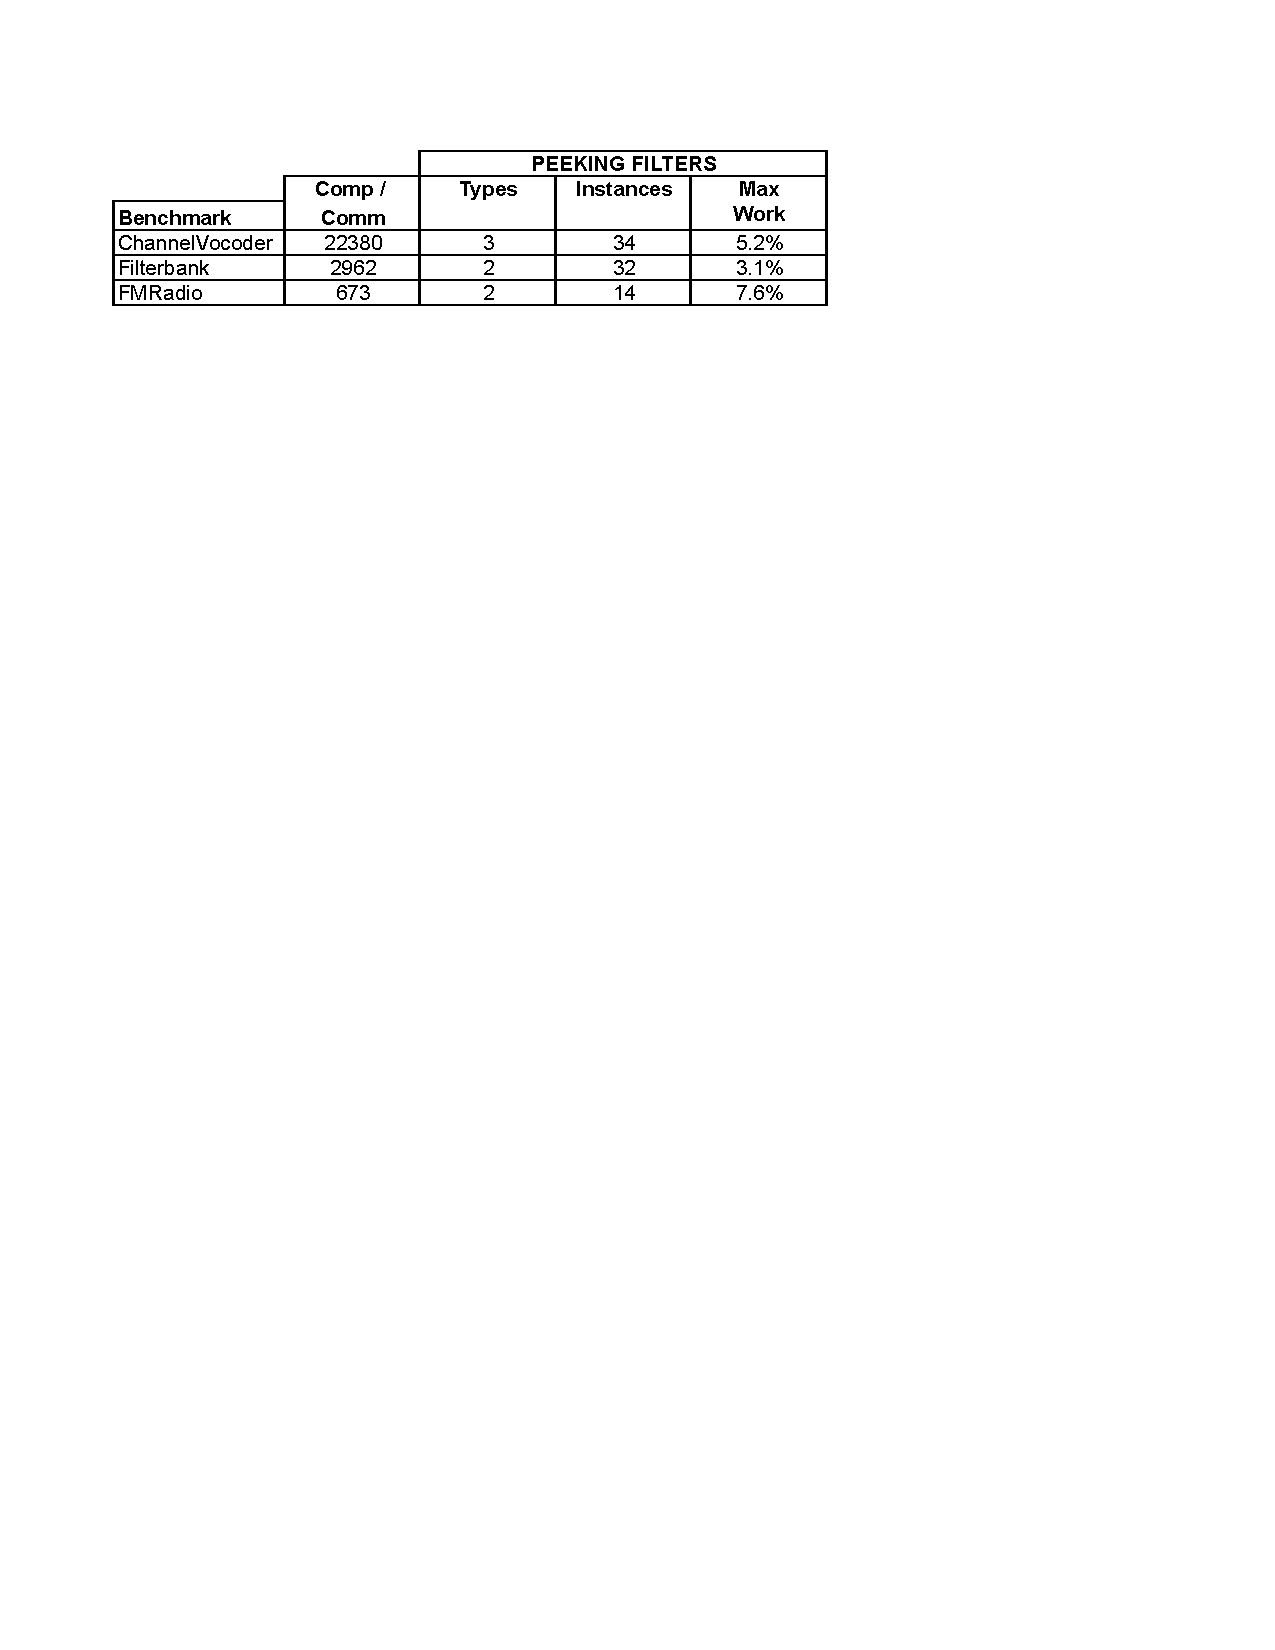
\includegraphics[width=3.3in]{figures/bench-char.pdf}}

In the above table, ``Comp/Comm'' provides a static estimation of the
amount of computation to communication ratio by statically estimating the total
work of all the filters and dividing by the number items communicated
for the programmer-conceived graph's steady-state.  The remaining
statistics give the number of peeking filters types, number of peeking
filters instantiated at runtime, and a static estimation of the max
work in the single most loaded peeking filter.

We target 2 multicore architecture with different communication
mechanisms.  The Tilera Corporation's TILE64 Processor is a 64 core
system on a chip~\cite{tilera}.  Each core is an identical three-wide
VLIW capable of running SMP Linux. The code generated by the StreamIt
compiler for the TILE64 processor follows the remote store programming
(RSP) model~\cite{rsp10} in which each process has a private address
space, but each process can award remote processes write access to
their local memory. When a producer process has write access to a
consumer process's memory, the producer communicates directly with the
consumer via store instructions whose destination is an address in the
consumer's shared memory.  Communication is initiated by the producer,
and is fine-grained.  The consumer reads directly from it's local
memory (L2) when accessing input.

Our symmetric multiprocessor target is a 16-core architecture that is
comprised of four Intel Xeon E7350 multicore processors.  Each processor
is a 64-bit, quad-core with two dual-core dies.  Each die contains a 4
MB L2 cache shared across the two cores.  The front-side bus is clocked
at 1066 MHz.  We utilize the cache coherency mechanism of the
architecture for communication between cores. 

\begin{figure*}[t]
\centering
\subfigure[]{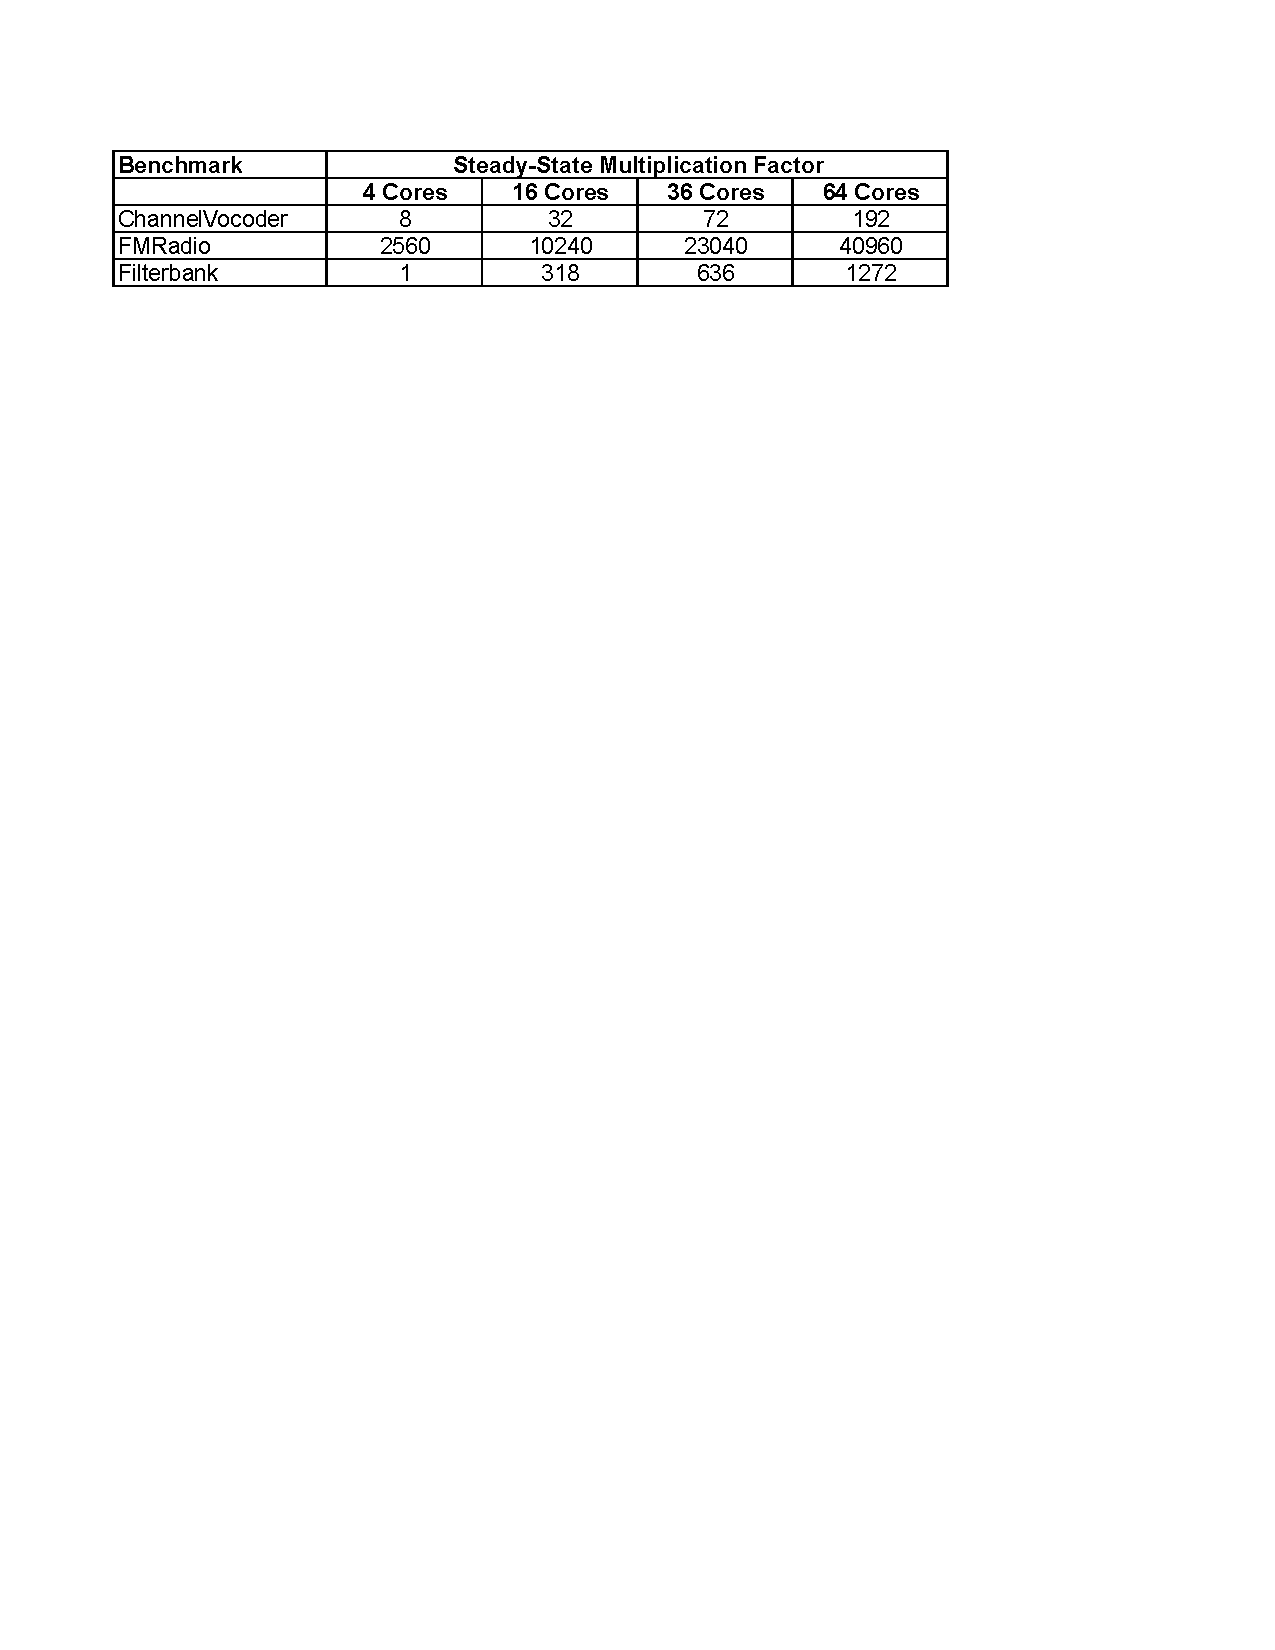
\includegraphics[width=3.7in]{figures/mult-table.pdf}} \\
\subfigure[]{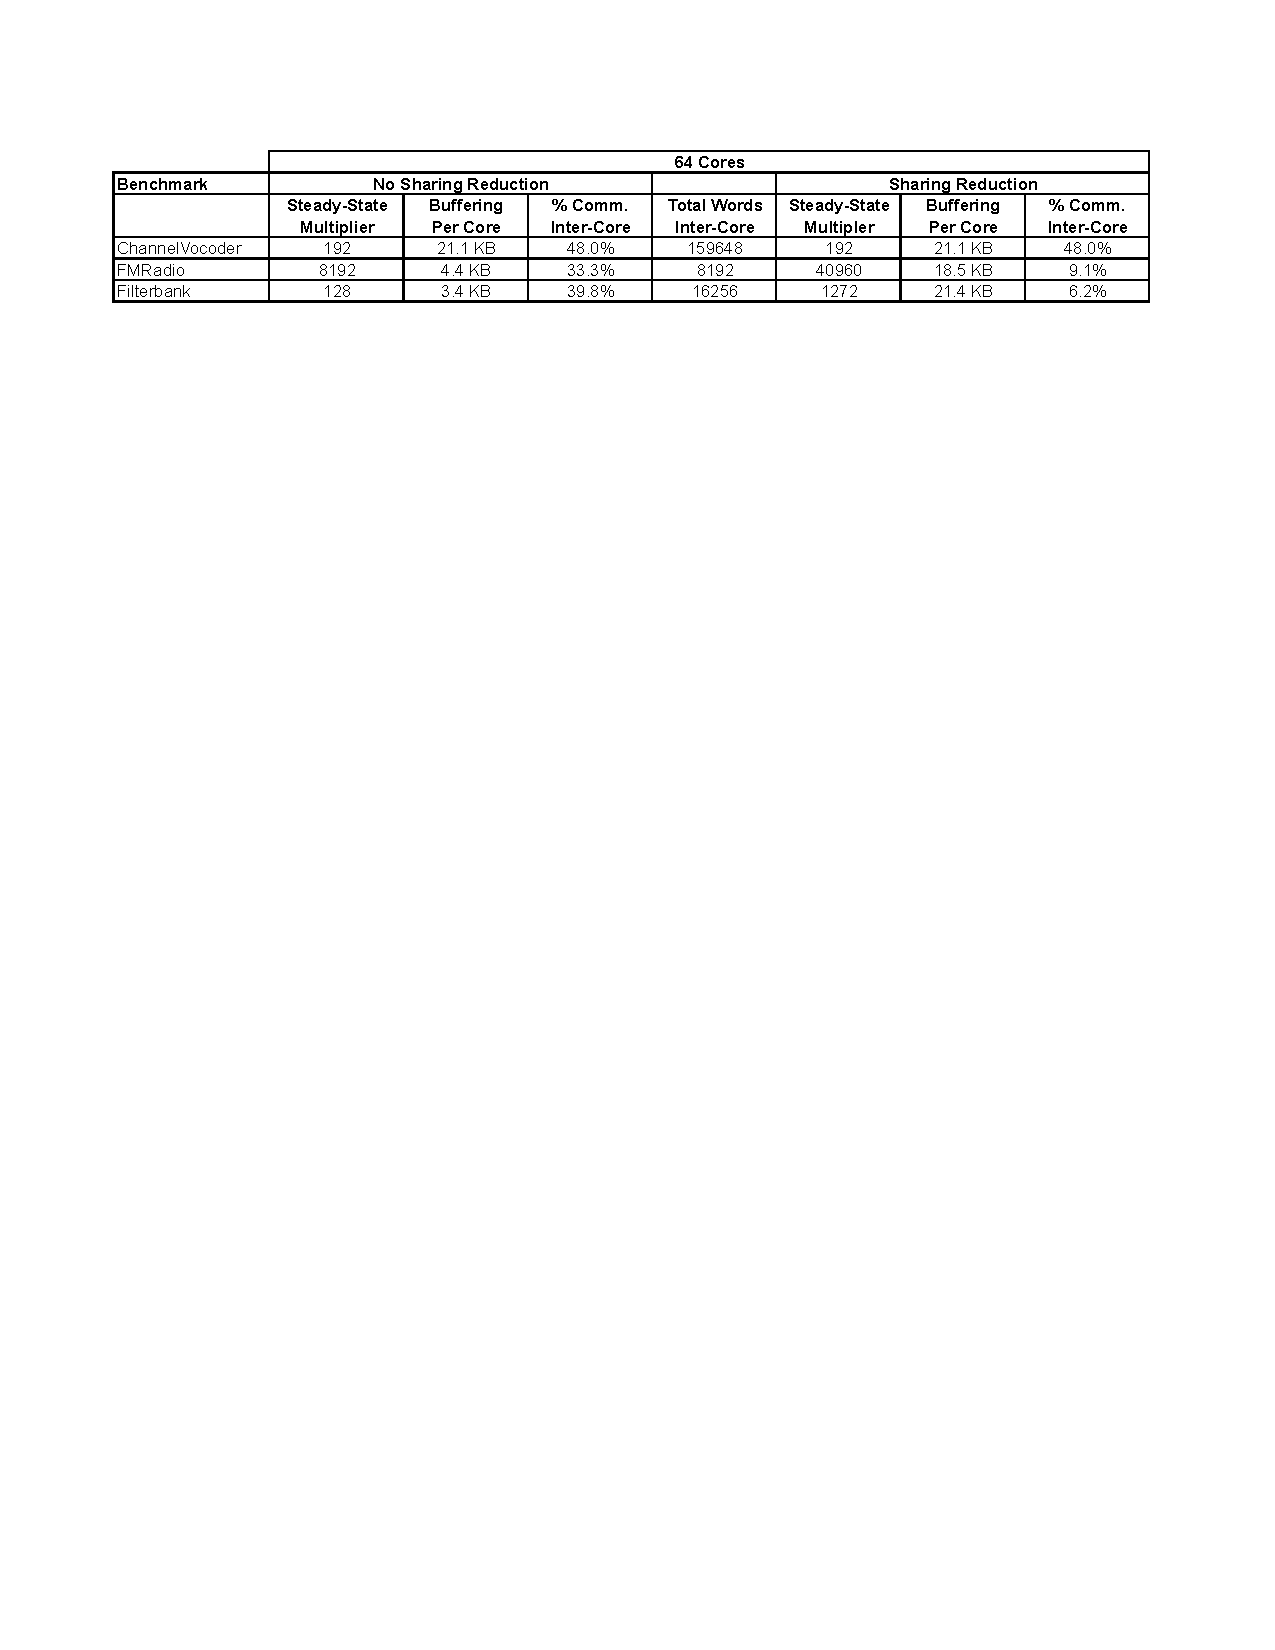
\includegraphics[width=6in]{figures/64-core-table.pdf}}
\caption[Communication, multiplier and buffering statistics for
benchmarks.]{
Communication, multiplier and buffering characteristics for
benchmarks: (a) gives the steady-state multipliers calculated for
sharing reduction, (b) compares the steady-state with and without
sharing reduction. 
\label{fig:fission-table}}
\end{figure*}

Figure~\ref{fig:fission-table}(a) gives the constant $c$
calculated for ChannelVocoder, Filterbank, and FMRadio for 4, 16, 36,
and 64 cores with: $T_{\mt{sharing}} = 0.10$ and $T_{\mt{apply}} =
0.05$.  The factor is larger for FMRadio because one filter
has $C(f) \gg o(S, f)$.  The multiplication factor affects both
latency and buffer sizes adversely.  The application designer will
have to decide if the latency of these techniques can be borne given
the application criteria.  The total buffering requirement is
increased when the steady-state is increased.  However, since we are
then fissing, the buffer is divided amongst the fission products, and
the {\it per-core} buffering requirement is unaffected by the
increase.  For example, FMRadio, has a per-core 18 KB buffering
requirement across all configurations (4, 16, 36, and 64 cores).  This
requirement fits in the per-core L2 size of 64 KB for the Tile64.

Figure~\ref{fig:fission-table}(b) compares the steady-state with and
without sharing reduction for a 64-core mapping.  For ChannelVocoder,
sharing reduction has no effect because most of the peeking filters do
not satisfy $T_{\mt{apply}} = 0.05$.  For the peeking filters that do,
the steady-state multiplier required for legal general fission for the
graph is enough to assure $T_{\mt{sharing}}$ is met.  Even though
sharing reduction has no effect for ChannelVocoder, general fission
avoids the 38\% of total items that were unnecessary duplicated by
DupDec.

For FMRadio and Filterbank, sharing reduction leads to significant
decreases in the percentage of total items communicated inter-core for
each steady-state.  The buffer requirement is increased an average of
5.2x for these benchmarks.  The total number of words communicated
inter-core during each steady-state is the same, with and without
sharing reduction.  However, the steady-state is greater in the
sharing reduction case, thus producing more outputs.

\begin{figure}[t]
\centering
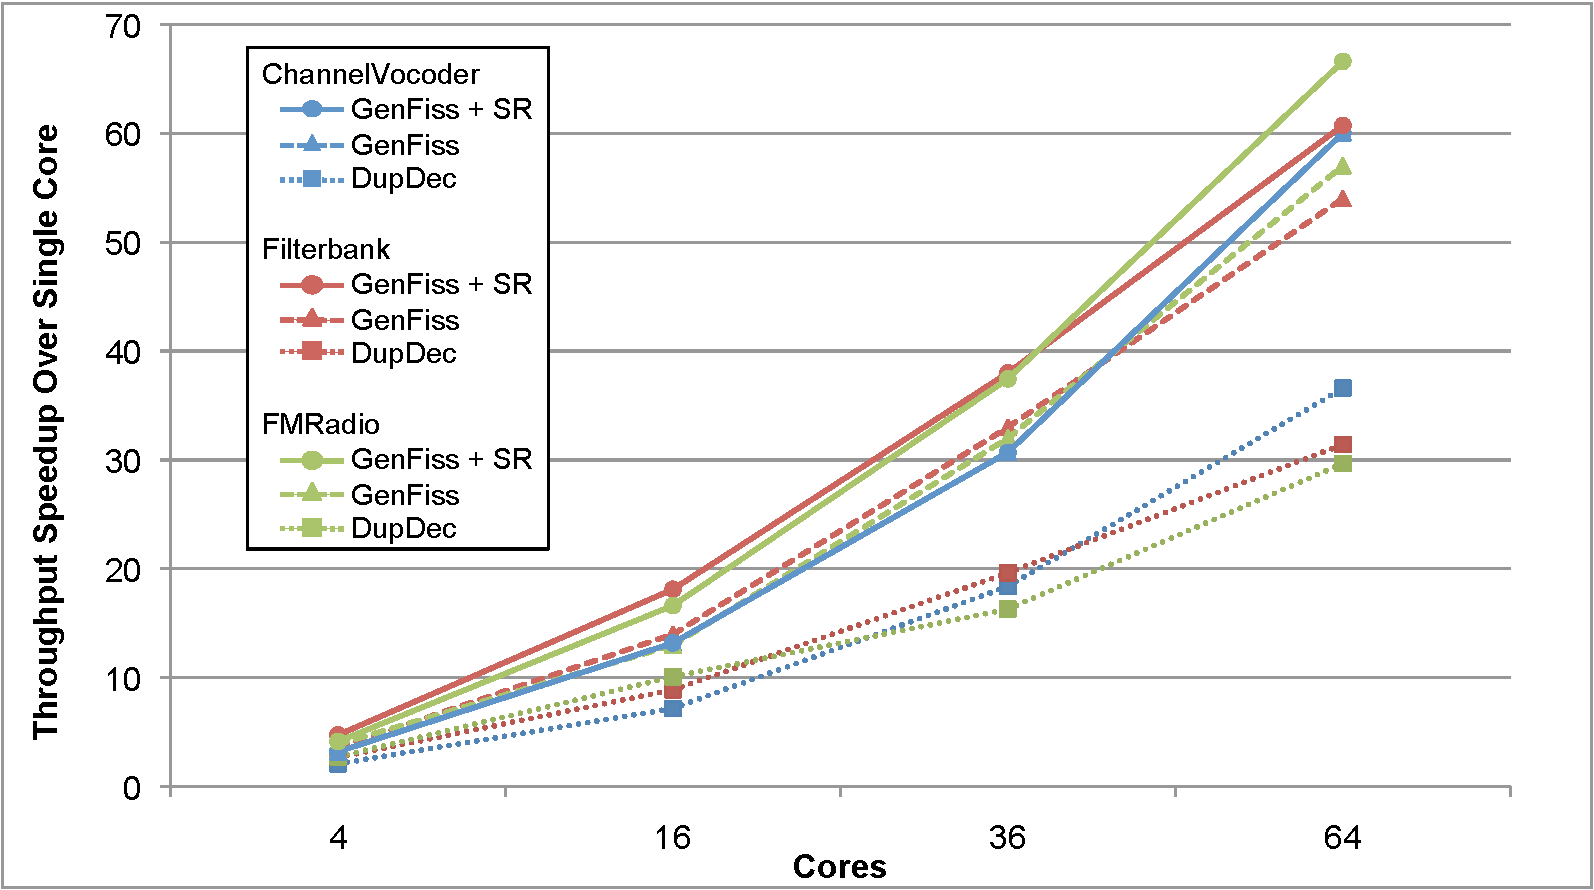
\includegraphics[width=3.3in]{figures/tilera-chart.pdf}
\caption[Comparing the fission techniques on the TILE64.]{
  Evaluation for DupDec versus general fission versus general fission with sharing reduction
  4, 16, 36, and 64 cores on the TILE64.  \label{fig:tilera-chart}}
\end{figure}

Figure~\ref{fig:tilera-chart} gives the performance results for the
Tilera TILE64 architecture.  We present results for DupDec, general
fission, and general fission with sharing reduction for 4, 16, 36, and
64 core configurations, with throughput normalized to single-core
throughput.  General fission with sharing reduction outperforms
dupdec by an average of 1.9x for the three benchmarks when targeting
64 cores. The average 64-core speedup over single core is 61x for the
general fission plus sharing reduction for these three benchmarks.

FMRadio experiences the most significant gain from general fission
plus sharing reduction over dupdec.  FMRadio has the lowest
computation to communication ratio of the 3 benchmarks.  Furthermore,
each filter of is fissed by the number of cores targeted.  For 64
cores, each filter is fissed 64 ways.  Dupdec must perform a global
all-to-all communication involving all 64 cores between each level of
the graph!  Conversely, general fission results in near-neighbor
communication in a ``snake'' across the 64 cores.  Dupdec achieves
only a 30x speedup for 64 cores while general fission plus sharing
reduction achieves a 67x speedup for 64 cores.

For ChannelVocoder achieve a 60x speedup for general fission over a
single core because the bottleneck for the application is a single
filter.  However, since the width of many of the other fission
applications is 3, DupDec is duplicating this input data to groups of
3 filters.  Thus the speedup for general fission over dupdec for
ChannelVocoder (1.62x) is not as great as compared to FMRadio when
dupdec duplicates to all 64 cores.  Filterbank is similar, the width
of fission is 4 for all filters when targeting 64 cores.

Sharing reduction is required to achieve scalable speedups for both
FMRadio and Filterbank.  For FMRadio, sharing reductions leads to a
17\% speedup increase for 64 cores.  This because sharing reduction
significantly reduces the number of remote write store instructions
required per output.  This affects FMRadio because of its low
computation to communication ratio.  Furthermore, the communication in
FMRadio is completely hidden by computation once sharing reduction is
enabled.  Sharing reduction sees a modest 12\% increase on Filterbank,
as Filterbank has a larger computation to communication ratio.

\begin{figure}[t]
\centering
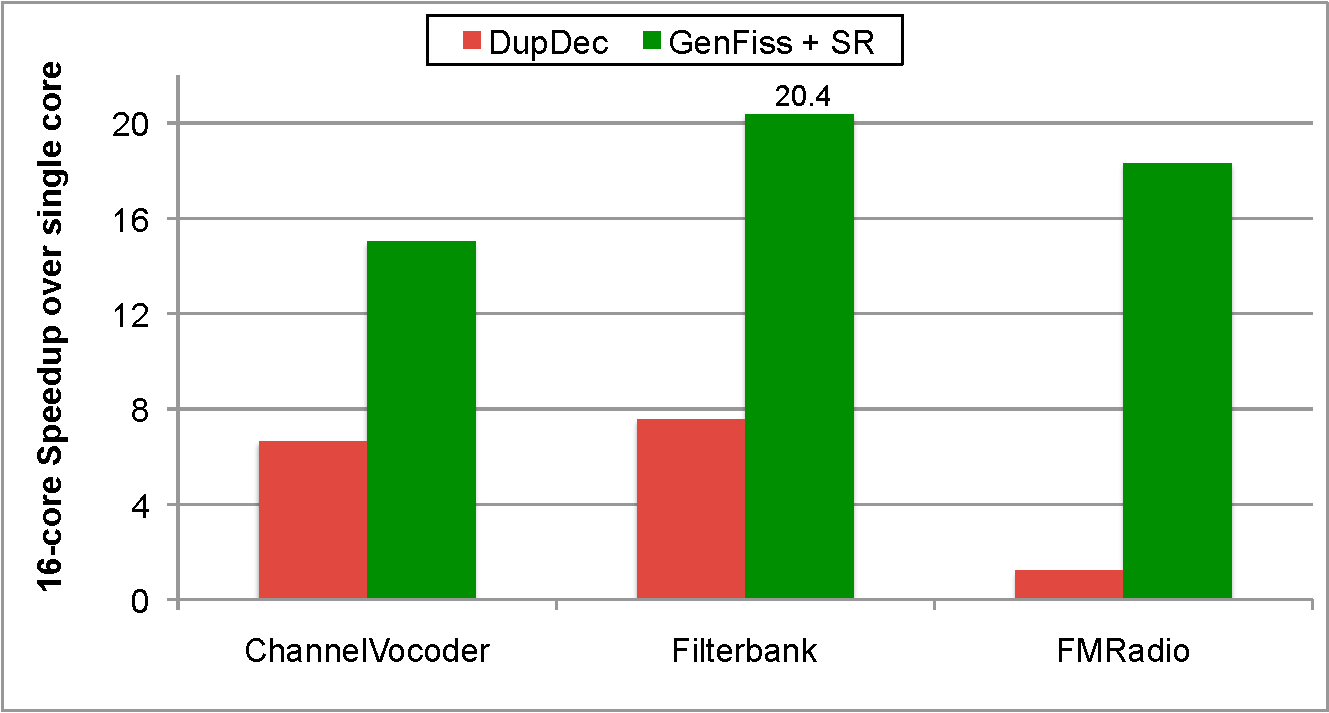
\includegraphics[width=3.3in]{figures/smp-chart.pdf}
\caption[Comparing the fission techniques on the 16-core SMP.]{
  Evaluation for DupDec versus general fission with sharing reduction
  for the 16-core SMP architecture.  \label{fig:smp-chart}}
\end{figure}

Figure~\ref{fig:smp-chart} gives the 16-core speedup comparison for
dupdec versus general fission with sharing reduction for our target
SMP architecture.  Concentrating on the benefit of general fission,
the average speedup increase for general fission with sharing
reduction over dupdec for peeking benchmarks (ChannelVocoder,
FilterBank, FMRadio, and Vocoder) is 5.5x.  FMRadio again sees the
largest speedup increase in the comparison at 13.0x.  The reasons for
this large speedup are similar as given in the previous section.
However, the SMP communication mechanism is not as efficient as the
TILE64, thus general fission gives a greater speedup.

summary paragraph...
